This section delineates the varied user personas that will interface with the \textbf{iBrief} application. It outlines their primary responsibilities and interactions with the system.

\begin{itemize}
    \item \textbf{End-Users (Citizens)}: These are general users concerned about urban aspects and public infrastructure. They utilize mobile devices to report issues and may appreciate incentives for their efforts. Their primary interactions involve:
        \begin{itemize}
            \item Reporting city-related issues.
            \item Tracking the status of their reports.
        \end{itemize}

        Figure \ref{fig:user-is-using-the-app} shows steps that a user follows for reporting an issue.
        \newpage
        \begin{figure}[!ht]
            \centering
            \caption{User is using the application}
            \label{fig:user-is-using-the-app}
            \begin{minipage}{0.4\textwidth}
                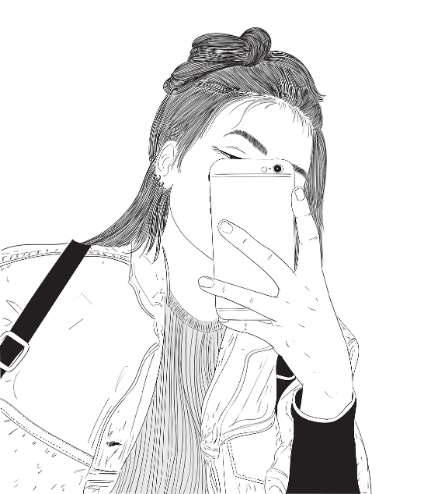
\includegraphics[width=\linewidth]{images/Image_ (1).png} 
            \end{minipage}%
            \hspace{0.05\textwidth} % Space between the image and the text
            \begin{minipage}{0.5\textwidth}
                I like to use my smartphone to take a picture and report this issue!
                \begin{enumerate}
                    \raggedright
                    \item Just open the app.
                    \item Make a new report.
                    \item Add address or use Geo location information.
                    \item If the city does not supported you will be informed, otherwise:
                    \item Select a category.
                    \item Add multimedia (i.e., picture, video, voice).
                    \item Press on submit button.
                    \item You will be updated regarding the progress.
                \end{enumerate}
            \end{minipage}
        \end{figure}

    \item \textbf{Officers (Local Authorities)}: Officers oversee all reported issues, ensuring timely and efficient resolution. Their responsibilities encompass:
        \begin{itemize}
            \item Monitoring all reports.
            \item Exporting report data.
            \item Integrating workflows with other applications.
        \end{itemize}

    \item \textbf{Agents (Issue Resolvers)}: Agents are tasked with the on-ground resolution of reported issues. Their workflow includes:
        \begin{itemize}
            \item Visiting reported locations.
            \item Updating the report's status throughout the resolution process.
        \end{itemize}

    \item \textbf{Administrators (Customer Point of Contacts)}: Administrators hold the highest permissions within their organization, acting as liaisons between the local authority and the \textbf{iBrief} team. They are accountable for:
        \begin{itemize}
            \item Contract management.
            \item Granting permissions.
            \item Configuring application workflows.
        \end{itemize}

    \item \textbf{Support Team}: Supports assist both the end-users and officers in using the application. They can:
        \begin{itemize}
            \item Address application-related queries.
            \item Escalate technical issues to developers.
        \end{itemize}

    \item \textbf{Sales Team}: Holding superior permissions than the support team, the sales team's responsibilities include:
        \begin{itemize}
            \item Customer relationship management.
            \item Contract preparation.
            \item Account management.
        \end{itemize}

    \item \textbf{Super Users (Developers and QA Team)}: Possessing the apex level of permissions, super users can:
        \begin{itemize}
            \item Access all system features.
            \item Test and validate application functionalities.
            \item Toggle between various roles for testing purposes.
        \end{itemize}
\end{itemize}
